
\subsection{Location and scale parameters for Cauchy data} \label{sec:cauchy}
%\ST{Main points: same results for ISABC and ACC with median because of BvM theorem; different results for mean but valid results for ACC due to pivot theorem}

In the Cauchy example presented in Figure \ref{fig:ACC} we saw how the lack of a sufficient summary statistic can change the validity of inferential conclusions from an approximate Bayesian inference approach. 
%to Algorithm \ref{alg:rejACC}. 
Through a CD perspective however, the inferential conclusions from ACDC %Algorithm \ref{alg:rejACC} 
are valid under the frequentist criterion even if the summary statistic is not sufficient. Provided Condition 1 is satisfied, different summary statistics produce different CDs. Here we present a continuation of this Cauchy example where random data ($n=400$) is drawn from a $Cauchy(\theta, \tau)$ distribution with data-generating parameter values $(\theta_0,\tau_0)=(10,0.55)$. We investigate the performance of $500$ independent $95\%$ confidence intervals for $\theta$ alone (settings one and two) and $\tau$ alone (setting three) and $500$ independent $95\%$ confidence regions when both parameters are unknown (settings four and five). 


%with this example to demonstrate the distinctions between these two approaches and to illustrate the potential gain in efficiency of a CD based approach over approximate Bayesian computing. In each of the five experimental settings discussed next, 
%Rather than draw comparisons to the Bayesian version of Algorithm \ref{alg:rejACC} with a flat prior, we consider the more level comparison between the performance of Algorithm \ref{alg:rejACC} and Algorithm \ref{alg:ISABC} (with a flat prior). (Simulations not presented here indicate that the results for a Bayesian version of Algorithm \ref{alg:rejACC} are similar to those of Algorithm \ref{alg:ISABC} but with a much smaller acceptance rate.) 


In each setting, the confidence intervals (regions) are generated for both accept-reject ACDC and IS-ABC utilizing the same 
%Algorithm \ref{alg:rejACC} and Algorithm \ref{alg:ISABC}. For each setting, the 
minibatch scheme to construct $r_n$ with the median and/or the median absolute deviation (MAD) as point estimators and $v=1/2$. The main difference in the two algorithms is the use of $r_n$. In former %Algorithm \ref{alg:rejACC}, 
$r_n$ is a data-driven initial CD estimate whereas 
%in Algorithm \ref{alg:ISABC}, we adapt a 
the latter represents a Bayesian approach that assumes an uninformative prior on the parameter space and employs $r_n(\theta)$ as the proposal distribution for the importance sampling updates. Both algorithms are improved by adapting the regression adjustments mentioned in Section \ref{sec:large_n_theory}, so the output for every run of each algorithm is post-processed in this manner. 

Table \ref{EX1_results} compares frequentist coverage proportions of confidence regions from both algorithms. The acceptance proportion determines how many simulated parameter values are kept and thus is directly related to the tolerance level. Most coverage rates are close to the nominal levels when the acceptance proportion is small, which is expected from the asymptotic theory in Section 3. Overall the coverage performance is similar for both algorithms. For settings one, three, and five with informative summary statistics, both algorithms give similar confidence regions which undercover a bit in the finite-sample regime. For settings two and four with less informative summary statistics, accept-reject ACDC %Algorithm \ref{alg:rejACC} 
is preferable because it produces tighter confidence bounds. 

\begin{table}
\caption{{\it Coverage proportions of confidence sets from ACDC applied to Cauchy data under five different settings. Coverage is calculated over $500$ independent runs that draw a $n=400$ IID sample from a $Cauchy(\theta = 10, \tau = 0.55)$ distribution. The Monte Carlo sample size for both %Algorithm \ref{alg:rejACC} and Algorithm \ref{alg:ISABC} 
algorithms is $50,000$ and the nominal coverage level in every setting is $95\%$. The last column displays the median ratio of the sizes of confidence sets from accept-reject ACDC 
%Algorithm \ref{alg:rejACC} 
divided by those from IS-ABC. }} 
\resizebox{0.5\textwidth}{!}{
\begin{tabular}{lllll}
\hline
\textbf{}                               & \textbf{Acceptance} & \textbf{ACDC}    & \textbf{IS-ABC}  & \textbf{Ratio of Widths/}     \\
                                        & \textbf{proportion} &  \textbf{Coverage}    &   \textbf{Coverage}   & \textbf{Volumes}              \\ \hline
\multicolumn{5}{l}{\textbf{Setting 1: $\theta$ unknown}}         \\ \hline
$S_n = Median(x)$                                                        & $0.005$             & $0.93$             & $0.94$         & $0.94$               \\
                                                                         & $0.05$              & $0.94$             & $0.94$        & $0.94$                \\
                                                                         & $0.10$              & $0.93$             & $0.94$        & $0.94$                \\ \hline
\multicolumn{5}{l}{\textbf{Setting 2: $\theta$ unknown}}                                                                                                                                          \\ \hline
$S_n = \bar{x}$                                                          & $0.005$             & $0.97$             & $0.98$         & $0.65$               \\
                                                                         & $0.05$              & $0.97$             & $0.98$        & $0.60$                \\
                                                                         & $0.10$              & $0.97$             & $0.98$        & $0.56$                \\   \hline
\multicolumn{5}{l}{\textbf{Setting 3: $\tau$ unknown}}                                                                      \\ \hline
$S_n = MAD(x)$                                                           & $0.005$             & $0.93$             & $0.94$         & $1.00$               \\
                                                                         & $0.05$              & $0.92$             & $0.94$        & $1.00$                \\
                                                                         & $0.10$              & $0.93$             & $0.94$        & $1.00$                \\ \hline
\multicolumn{5}{l}{\textbf{Setting 4: $(\theta, \tau)'$ both unknown}}               \\ \hline
\multirow{2}{*}{$S_n = \begin{pmatrix} \bar{x} \\ SD(x)\end{pmatrix}$}   & $0.005$             & $0.96$             & $0.96$         & $0.58$               \\
                                                                         & $0.05$              & $0.99$             & $0.98$        & $0.48$                \\
                                                                         & $0.10$              & $0.99$             & $0.98$        & $0.47$                \\ \hline
\multicolumn{5}{l}{\textbf{Setting 5: $(\theta, \tau)'$ both unknown}}          \\ \hline
\multirow{2}{*}{$S_n = \begin{pmatrix}Median(x) \\ MAD(x)\end{pmatrix}$} & $0.005$             & $0.91$             & $0.93$         & $0.98$               \\
                                                                         & $0.05$              & $0.94$             & $0.96$        & $1.00$                \\
                                                                         & $0.10$              & $0.94$             & $0.97$        & $1.00$                \\     
\end{tabular}\label{EX1_results}}
\end{table}

The main reason for the favorable performance of accept-reject ACDC 
%out-performance of Algorithm \ref{alg:rejACC} is the 
is related to the skewed importance weights for IS-ABC. This can be seen in the sizes of the confidence sets of the two algorithms in Table \ref{EX1_results} but is even more clear when comparing the CD densities of each method as in Figure \ref{fig:cauchy_loc_ex}. Figure \ref{fig:cauchy_loc_ex} shows the impact of importance weights in IS-ABC %Algorithm \ref{alg:ISABC} 
on the variances of point estimators and CDs. %, the latter of which is reflected by comparing the sizes of confidence sets from the two algorithms. 
For settings 1,3 and 5 where an informative summary statistic is used, the importance weights do not much affect either the point estimator or resulting CDs. In these cases, $r_n(\theta)$ is a good proposal distribution according to the criteria in \cite{Li2016}. For settings 2 and 4 however, where the summary statistic is less informative, Figure \ref{fig:cauchy_loc_ex} shows how the importance weights inflate both point estimate and CD variances with Monte Carlo variation in IS-ABC. One reason for the severe skewedness in the importance weights $\pi(\theta)/r_n(\theta)$ is that the high variance of $S_n$ means more parameter simulations are accepted in the tails of $r_n(\theta)$. This results in broader confidence regions for IS-ABC than accept-reject ACDC.

\begin{figure}
\centering
\caption{{\it These are densities of point estimators from accept-reject ACDC (red) and IS-ABC (black) for the $500$ independent data sets for each of the five settings in Table \ref{EX1_results}. Additionally, this figure shows a box plot of the relative sizes of the $500$ confidence sets, that is, the length (or volume) of regions produced by accept-reject ACDC %Algorithm \ref{alg:rejACC} 
divided by those of IS-ABC.}}\label{fig:cauchy_loc_ex}
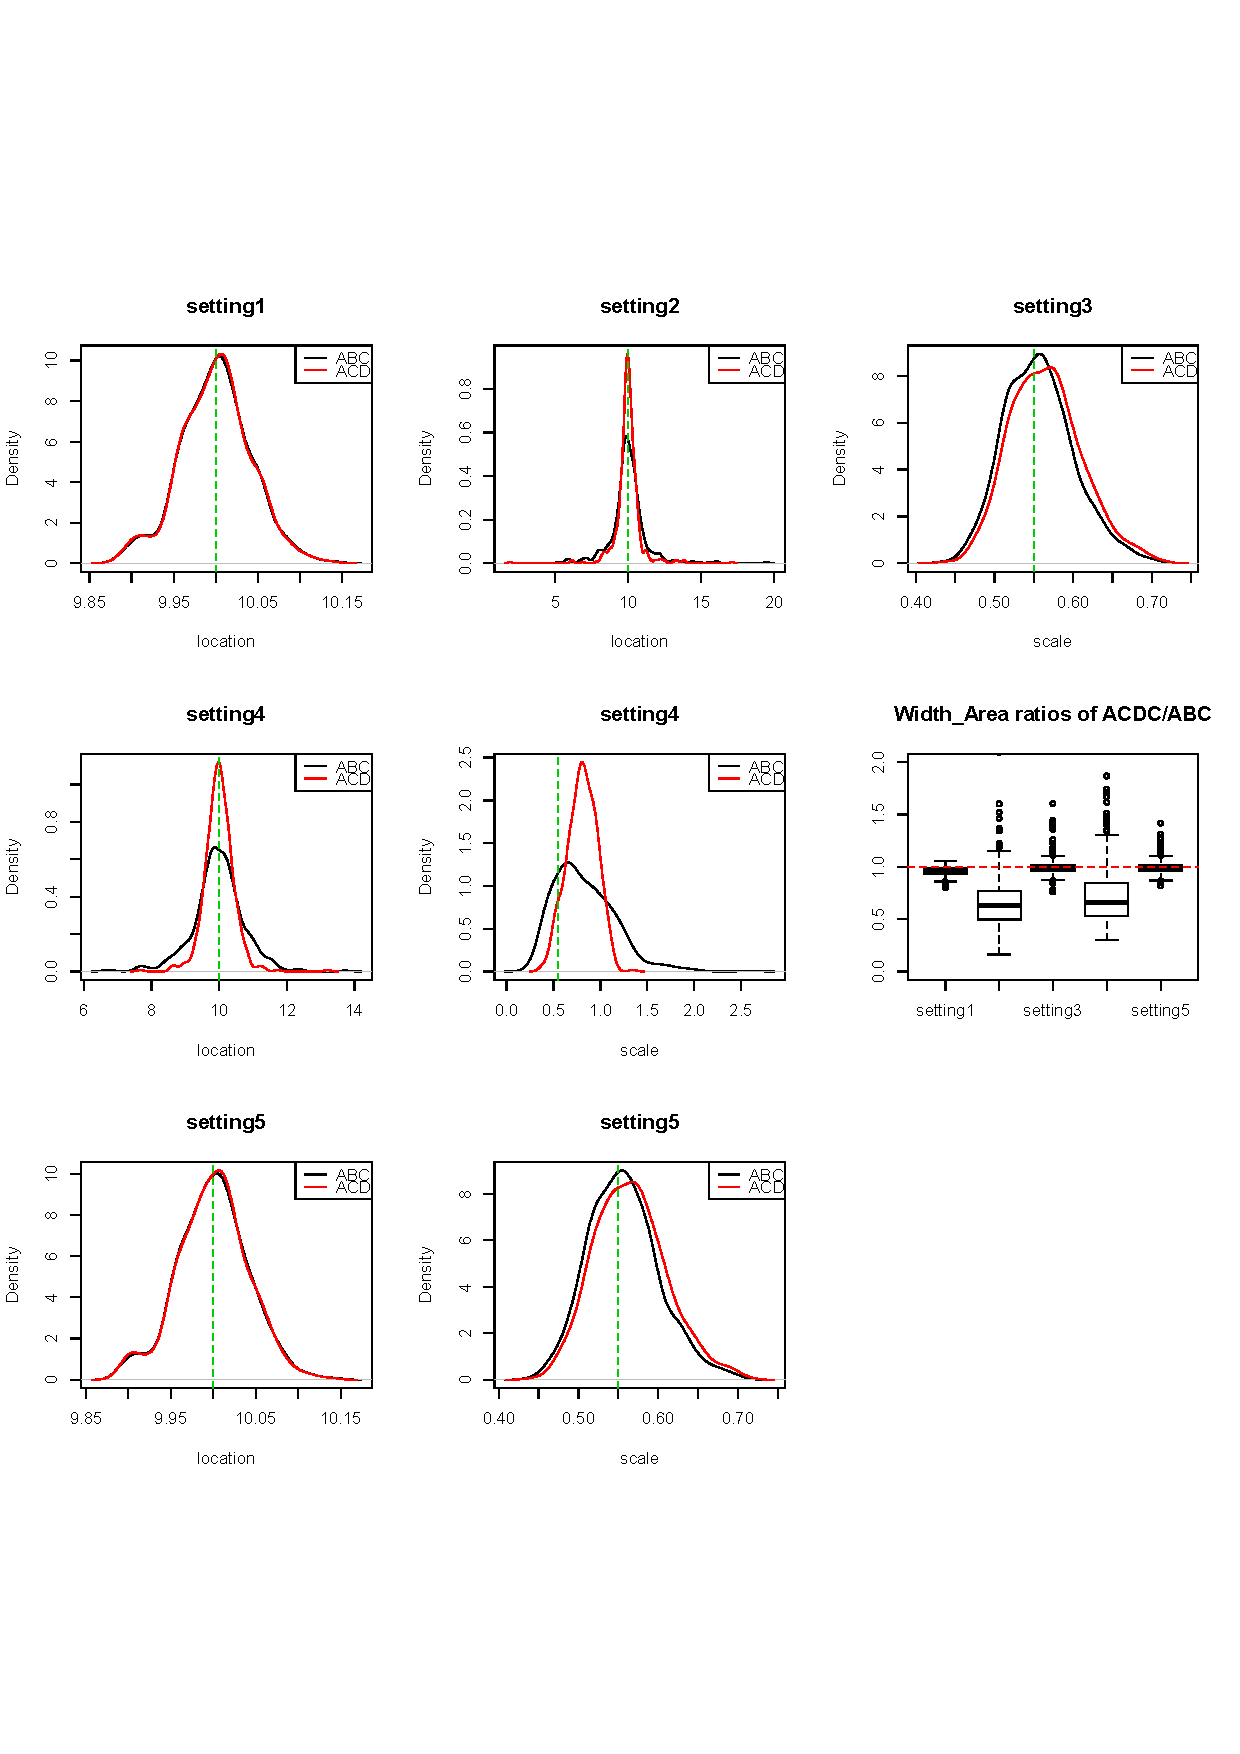
\includegraphics[width=0.9\linewidth]{Images/Cauchy_one_run.pdf}
\end{figure}	

This numerical study validates inference for both 
accept-reject ACDC and IS-ABC %Algorithms \ref{alg:rejACC} and \ref{alg:ISABC} 
%in terms of frequentest coverage rates, 
even in the case where typical asymptotic arguments do not apply (settings 2 and 4). 
Furthermore, this example demonstrates two valid but distinct uses of the minibatch scheme for constructing a data driven distribution estimator. In Algorithm \ref{alg:rejACC}, $r_n$ drives the search for a distribution estimator or acts as a data-dependent prior within a Bayesian context. In Algorithm \ref{alg:ISABC}, $r_n$ acts as a proposal distribution for ABC with a flat prior. The computational differences in the performance of confidence regions in this example suggest that the former application of $r_n$ is preferable to the latter if the summary statistic is not very informative. Interestingly, even though the Bayesian IS-ABC algorithm fails to give us Bayesian posterior distributions, it can still provide us valid frequentist inference.  


\subsection{Mulit-parameter inference for a Ricker model}\label{sec:ricker}
A Ricker map is a non-linear dynamical system, often used in Ecology, that describes how a population changes over time. The population, $N_t$, is noisily observed and is described by the following model,
\begin{align*}
	& y_t \sim \mbox{Pois}(\phi N_t),\\
	& N_t = r N_{t-1}e^{-N_{t-1}+e_t}, e_t\sim N(0,\sigma^2),
\end{align*}
where $t=1,\ldots,T$ and parameters $r$, $\phi$ and $\sigma$ are positive constants, interpreted as the intrinsic growth rate of the population, a scale parameter, and the environmental noise, respectively. This model is computationally challenging since its likelihood function is intractable for $\sigma > 0$ and is highly irregular in certain regions of the parameter space. 
%~\cite{wood2010statistical} suggests a summary statistic-based inference, instead of likelihood-based inference, to overcome the noise-driven nature of the model. ~\cite{Fearnhead2012} applies Algorithm \ref{alg:ISABC} with a regression adjustment to the above model and improvement over the Gaussian approximate-likelihood method of ~\cite{wood2010statistical}. More recently, \cite{Fasiolo2016} have compared many \ST{likelihood-free?} inferential methods for the Ricker model (among others). Their findings indicate that for both the Ricker and Generalized Ricker models, in terms of root-mean squared error, approximate Bayesian computation is the superior method for inference on the noise parameter $\sigma$. % However, in terms of coverage under repeated sampling, none of the methods (including approximate Bayesian computation) appear adequate. (See Tables 6 and 7 of the supplementary material for \cite{Fasiolo2016}.) %Wentao says this is because of computing issues, not theory issues 

We investigate the performance of confidence bounds for each parameter marginally and two pairs of parameters jointly. We follow the setting and the choice of summary statistics in \cite{wood2010statistical}. The output of both algorithms are post-processed using the regression adjustment.  

In the minibatch scheme, for the point estimator we use $E\{\theta\mid S_n(z_i)\}$ estimated by the population Monte Carlo version of IS-ABC. 
%Algorithm \ref{alg:ISABC}. 
The maximum synthetic likelihood estimator proposed in \cite{wood2010statistical} was also tried, but the estimates obtained this way over-concentrated in a certain area of the parameter space. The 
corresponding $r_n(\theta)$ did not cover the target mass very well, causing biases in the coverage levels. Instead, $r_n(\theta)$ is used to initialise the population Monte Carlo iterations. Since the sample size is small in this example, overlapping minibatches are chosen with a total number of $40$ where each minibatch contains a series of  length $10$. In this example, the parametric bootstrap method is not computationally feasible because it is computationally expensive to use the simulation-based methods in obtaining the point estimates.

In Table \ref{EX2_results}, when the acceptance proportion is small, most coverage rates of %Algorithm \ref{alg:rejACC} 
accept-reject ACDC are close to the nominal level. In contrast, the  confidence bounds from IS-ABC 
%Algorithm \ref{alg:ISABC} show 
display more over-coverage, indicating an even  smaller $\varepsilon$ is needed to reduce the variance inflation. Furthermore, all ACDC confidence regions %of Algorithm \ref{alg:rejACC} 
are tighter with a size reduction up to $51\%$. The box plots in Figure \ref{fig:EX2_results} show that the CD variances from IS-ABC are inflated substantially by the importance weights, resulting in broader confidence regions as observed in the last column of Table \ref{EX2_results}.
%As in Section \ref{sec:cauchy}, the boxplots in Figure \ref{fig:EX2_results} show that the variances of point estimators and CDs from IS-ABC 
%of Algorithm \ref{alg:ISABC} 
%are inflated substantially by the importance weights leading to the broader confidence regions observed in Table \ref{EX2_results}. 
%However, Algorithm \ref{alg:rejACC} can still avoid the excessive Monte Carlo variation that impedes Algorithm \ref{alg:ISABC}.

% As in the previous example, we investigate the performance of $95\%$ confidence intervals for each marginal parameter (Settings 1-3) and $95\%$ confidence regions for two joint-parameter cases (Settings 4-5). Since this numerical example is much more computationally costly, coverage is only computed over $150$ independent runs. Following \cite{wood2010statistical}, each data set is generated for parameter value $\theta_0=(e^{3.8},0.3,10)$ and contains observations from times $t=51$ to $100$. Both Algorithm \ref{alg:rejACC} and \ref{alg:ISABC} use the same 11-dimensional summary statistic and point estimate described in \cite{wood2010statistical}. Because this example involves a heavy computational cost in generating these complicated summary statistics and point estimates, the parametric bootstrap method is not computationally feasible in this example. 


%The six experimental settings for this example consider one and two dimensional inference for the unknown parameter $\theta=(r,\phi,\sigma)$ and compare the resulting distribution estimates from Algorithm \ref{alg:rejACC} and a population Monte Carlo version of Algorithm \ref{alg:ISABC}.\cite[]{Cappe2004} (Rather than simulating from the prior distribution, the population Monte Carlo algorithm is initialized from the proposal distribution using the maximum synthetic likelihood estimator established in ~\cite{wood2010statistical}.)  Table \ref{EX2_results} show the coverage results and relative interval/region size for each algorithm and each experiment. 
%% Need Wentao's help to rewrite these parts 
%{\it We use the minibatch scheme to choose $r_{n}(\theta)$ for both the initial density of Algorithm \ref{alg:rejACC} and the proposal density of Algorithm \ref{alg:ISABC}. Specifically, we obtain $\htheta$ with a mixture of a case-dependent point estimator and $E\{\theta\mid S_{n}(z_i)\}$. That is, $\htheta = E\{\theta\mid S_{n}(z_i)\}$, which is obtained from the population Monte Carlo version of an approximate Bayesian computing algorithm.~\cite[]{Cappe2004}  
%Rather than simulating from the prior distribution, the population Monte Carlo algorithm is initialized from the proposal distribution using the maximum synthetic likelihood estimator established in ~\cite{wood2010statistical}. 
%(Simulations not shown here implemented a minibatch scheme using the \ST{maximum (synthetic likelihood?) estimator} as $\htheta$ but this caused significant bias in the coverage for both algorithms.)}
%{\it The mixing procedure is a refinement of this method that adds several population Monte Carlo iterations after obtaining the \ST{maximum (synthetic likelihood?) estimator}. This refined version produces estimators with smaller bias and lower computational cost than implementations of these algorithms that rely on either point estimator individually. Additionally, the resulting confidence/credible intervals both have better coverage performance with tighter interval bounds. 

	
%To define $\r(\theta)$, each minibatch of the sample has size $10$ and a total number of $40$ batches are used \ST{rewrite in terms of $\delta$}. The mini-batches of the data are permitted to overlap in order to ensure a reasonable number of point estimates are available in the current small sample setting. 



\begin{table}
\caption{{\it Coverage proportions of marginal confidence intervals (or joint confidence regions) for accept-reject ACDC and IS-ABC applied to Ricker data. Coverage is calculated over $150$ independent runs that produce observations from $t=51$ to $100$ for data generated by a Ricker model with $(r,\sigma, \phi)=(e^{3.8},0.3,10)$. The Monte Carlo sample size for both algorithms is $50,000$ and the nominal coverage level in every setting is $95\%$. The last column displays the median ratio of the sizes of confidence sets from accept-reject ACDC divided by those from IS-ABC.}}
\resizebox{0.5\textwidth}{!}{
\begin{tabular}{lllll}
\hline
\textbf{}                               & \textbf{Acceptance} & \textbf{ACDC}    & \textbf{IS-ABC}  & \textbf{Ratio of Widths/}     \\
                                        & \textbf{proportion} &  \textbf{Coverage}    &   \textbf{Coverage}   & \textbf{Volumes}              \\ \hline
\multicolumn{5}{l}{\textbf{Setting 1: $log(r)$ unknown}}         \\ \hline
           & $0.005$            & $0.953$             & $0.980$       & $0.793$               \\
          & $0.05$              & $0.960$             & $0.987$        & $0.734$                \\
          & $0.10$              & $0.967$             & $0.987$        & $0.707$                \\ \hline
\multicolumn{5}{l}{\textbf{Setting 2: $log(\sigma)$ unknown}}              \\ \hline
          & $0.005$             & $0.967$             & $0.987$         & $0.782$               \\
          & $0.05$              & $0.987$             & $0.993$        & $0.732$                \\
          & $0.10$              & $0.987$             & $0.993$        & $0.717$                \\ \hline
\multicolumn{5}{l}{\textbf{Setting 3: $log(\phi)$ unknown}}               \\ \hline
          & $0.005$             & $0.953$             & $0.967$         & $0.828$               \\
          & $0.05$              & $0.947$             & $0.993$        & $0.762$                \\
          & $0.10$              & $0.960$             & $0.987$        & $0.734$                \\ \hline
\multicolumn{5}{l}{\textbf{Setting 4: $(log(r), log(\sigma))'$} unknown}               \\ \hline
          & $0.005$             & $0.960$             & $0.947$         & $0.611$               \\
          & $0.05$              & $0.960$             & $0.973$        & $0.519$                \\
          & $0.10$              & $0.960$             & $0.947$        & $0.484$                \\ \hline
\multicolumn{5}{l}{\textbf{Setting 5: $(log(r), log(\phi))'$ unknown}}          \\ \hline
          & $0.005$             & $0.973$             & $0.987$         & $0.749$               \\
          & $0.05$              & $1.0$             & $1.0$        & $0.619$                \\
          & $0.10$              & $1.0$             & $1.0$        & $0.557$                %\\ \hline
%\multicolumn{5}{l}{\textbf{Experiment 6: $(log(\sigma), log(\phi))'$ both unknown}}          \\ \hline
%         & $0.005$              & $x$             & $x$        & $x$           \\
%          & $0.05$              & $x$             & $x$        & $x$                \\
%          & $0.10$              & $x$             & $x$        & $x$                \\  
\end{tabular}\label{EX2_results}}
\end{table}


\begin{figure}
\centering
\caption{{\it These are densities of point estimators from accept-reject ACDC (red) and IS-ABC (black) for the $150$ independent data sets produced by the Ricker model. Additionally, this figure shows a box plot of the ratio of the sizes of the $150$ confidence sets, that is, the length (or volume) of regions produced by accept-reject ACDC divided by those of IS-ABC.
%confidence intervals (or regions) from both algorithms over $150$ independent data sets, that is the length (or area) of Algorithm \ref{alg:rejACC} divided by that of Algorithm \ref{alg:ISABC}.
}}\label{fig:EX2_results}
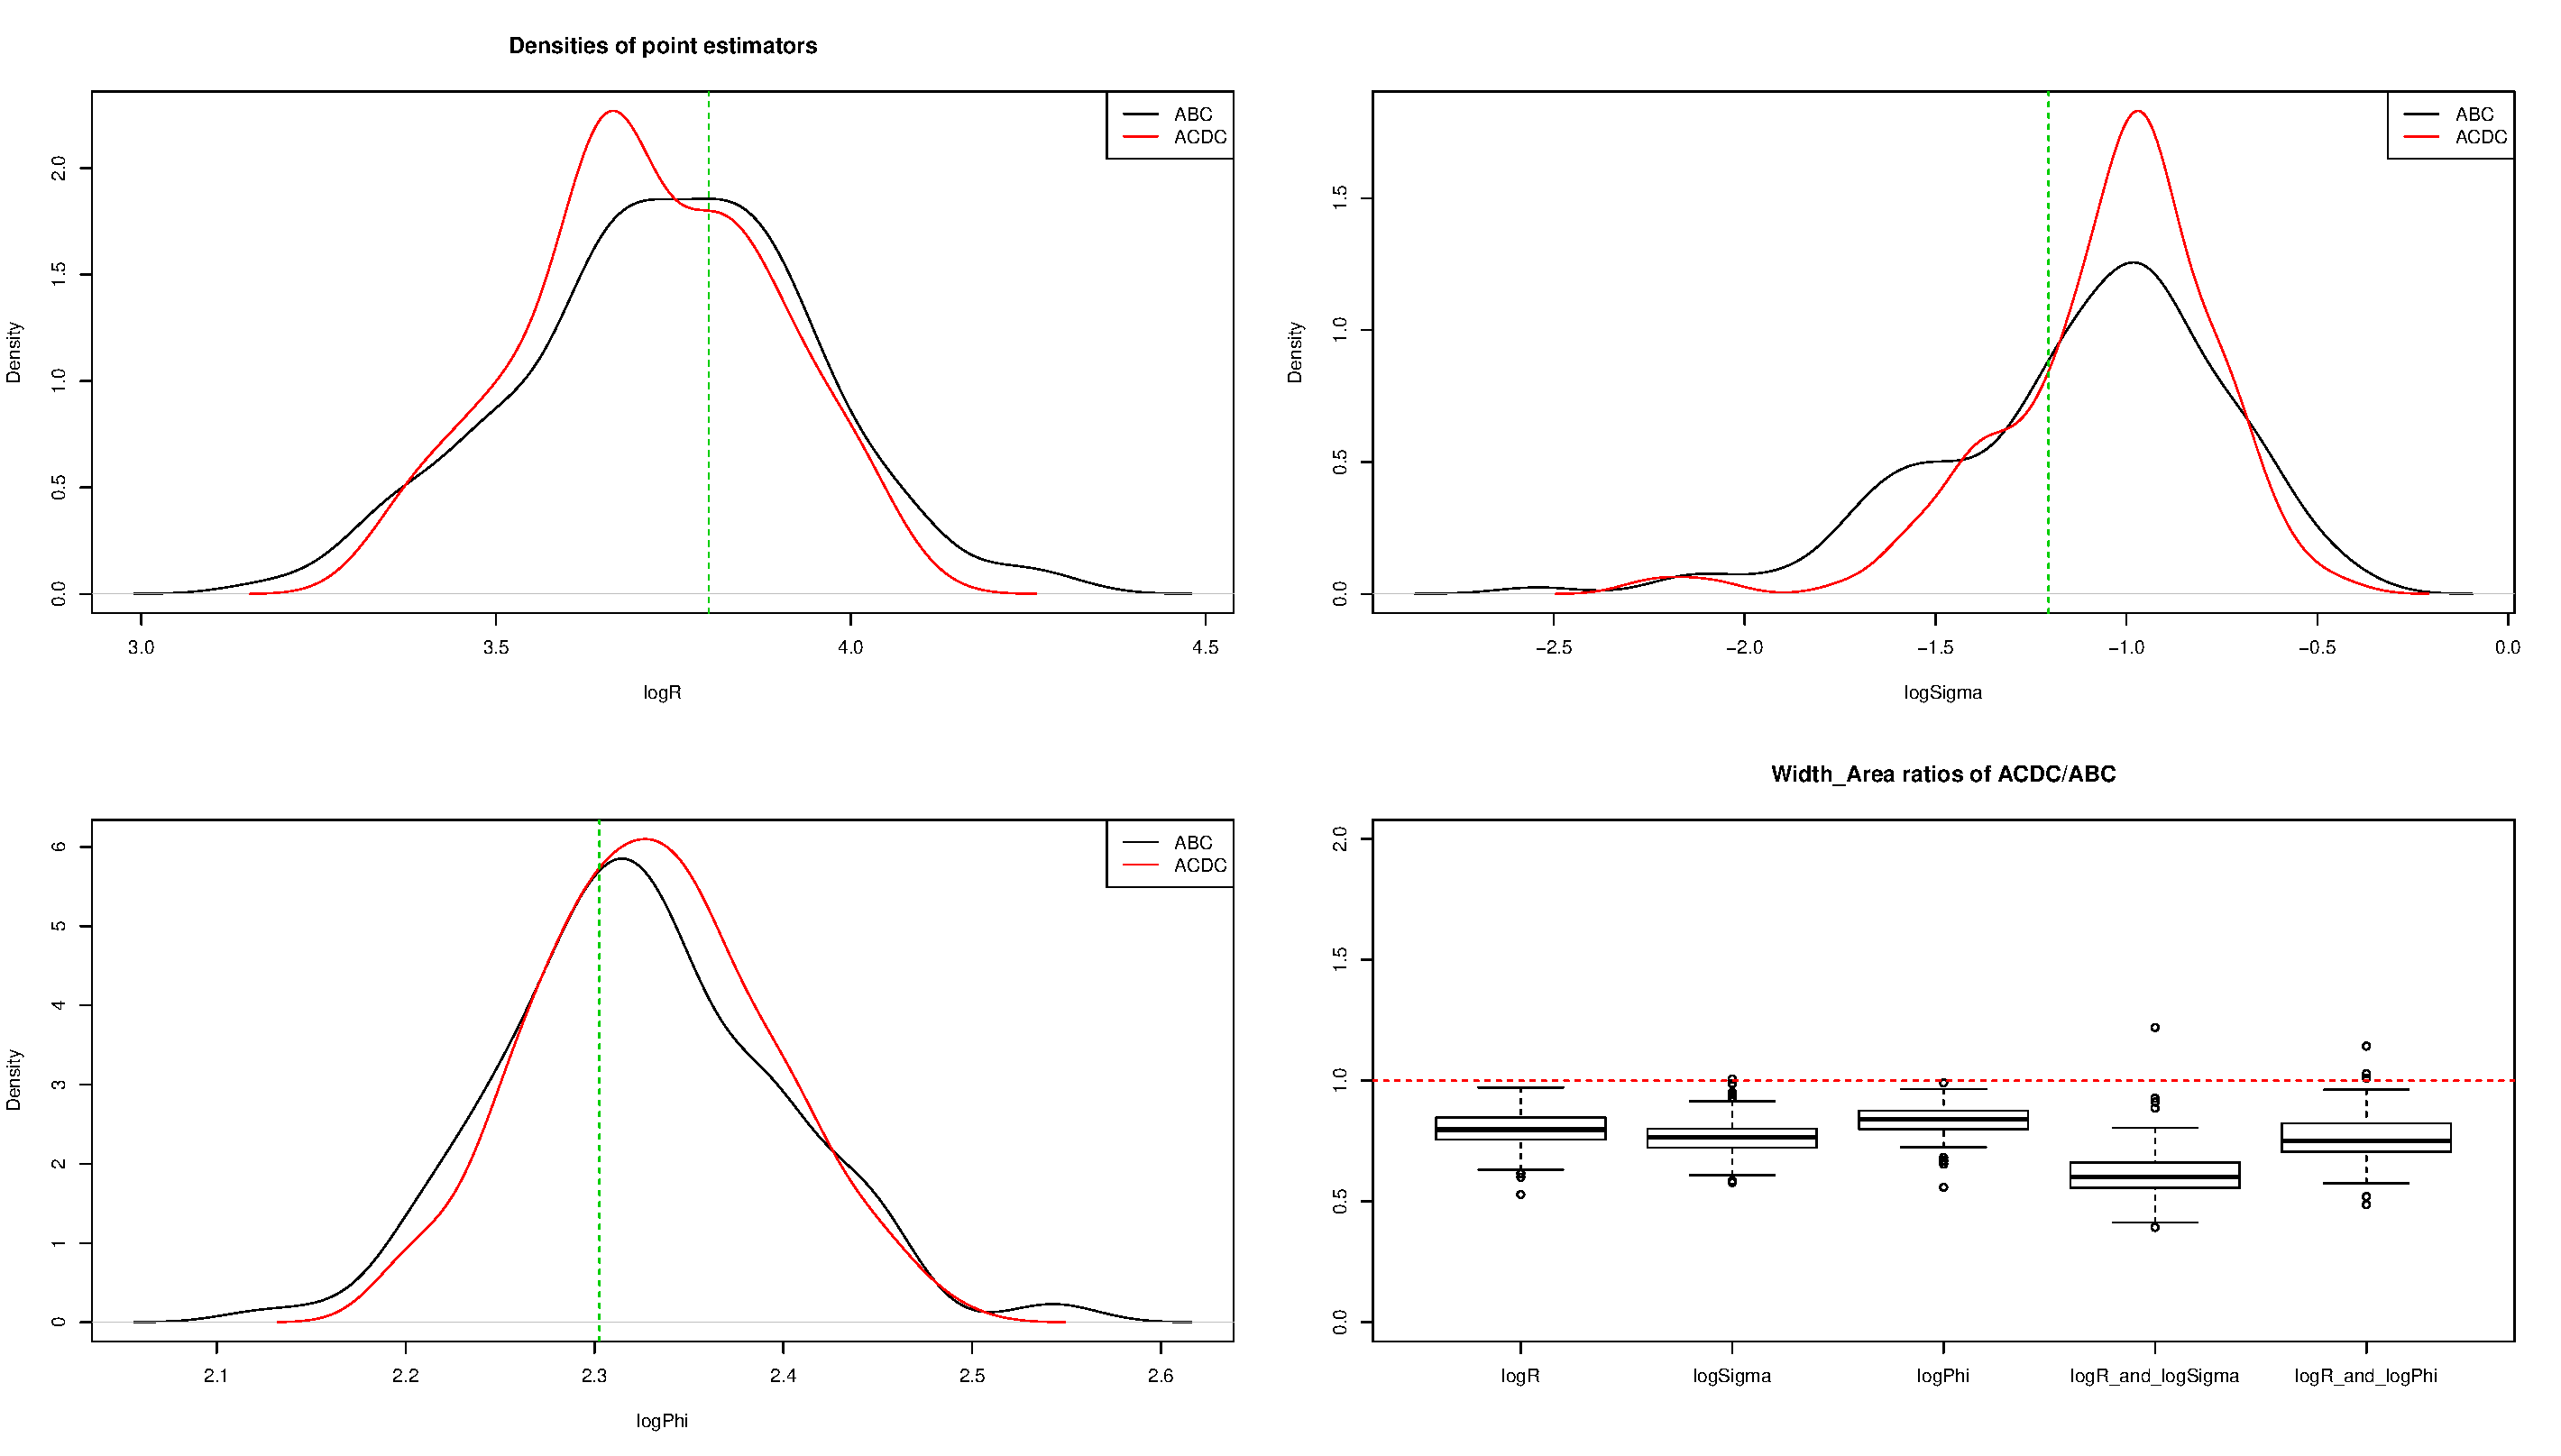
\includegraphics[width=0.9\linewidth]{Images/Ricker_one_run.pdf}
\end{figure}


As in Section \ref{sec:cauchy}, this numerical example validates the inferential conclusions from both algorithms but here we see accept-reject ACDC %that Algorithm \ref{alg:rejACC} 
consistently producing tighter confidence regions than IS-ABC. The summary statistics in this example were carefully selected to be informative based on domain knowledge. Nevertheless, accept-reject ACDC can still avoid the excessive Monte Carlo variation that impedes IS-ABC.


